% document formatting
\documentclass[10pt]{article}
\usepackage[utf8]{inputenc}
\usepackage[left=1in,right=1in,top=1in,bottom=1in]{geometry}
\usepackage[T1]{fontenc}
\usepackage{xcolor}

% math symbols, etc.
\usepackage{amsmath, amsfonts, amssymb, amsthm}

% lists
\usepackage{enumerate}

% images
\usepackage{graphicx} % for images
\usepackage{tikz}
\usetikzlibrary{intersections, calc}

% code blocks
% \usepackage{minted, listings} 

% verbatim greek
\usepackage{alphabeta}

\newcommand{\opt}{\texttt{OPT}}

\graphicspath{{./assets/images/Week 14}}

\title{02-613 Week 14 \\ \large{Algorithms and Advanced Data Structures}}
 
\author{Aidan Jan}

\date{\today}

\begin{document}
\maketitle

\subsection*{Using 3SAT to Prove NP-Hard}
3SAT has been proven to be NP-Hard (in fact, it was the first) in 1971 in the Cook-Levin paper.  Now we can use it in other proofs.

\subsubsection*{Proving Independent Set is NP-Hard}
We can reduce 3SAT to Independent Set to show that Independent Set is NP-Hard.  To do this, draw a graph.  Each clause of three terms OR'ed together is converted to 3 nodes on the graph connected with edges.  Furthermore, each node that reference the same term (e.g., if $t_1$ is in two different clauses), the two nodes are also connected with an edge.  Now, this is an independent set problem, where whichever nodes are set to true are possible values that would satisfy 3SAT.\\\\
For example, consider $(x_1 \lor x_2 \lor \overline{x_3}) \land (x_2 \lor x_3 \lor \overline{x_4}) \land (x_1 \lor \overline{x_2} \lor x_4)$
\begin{center}
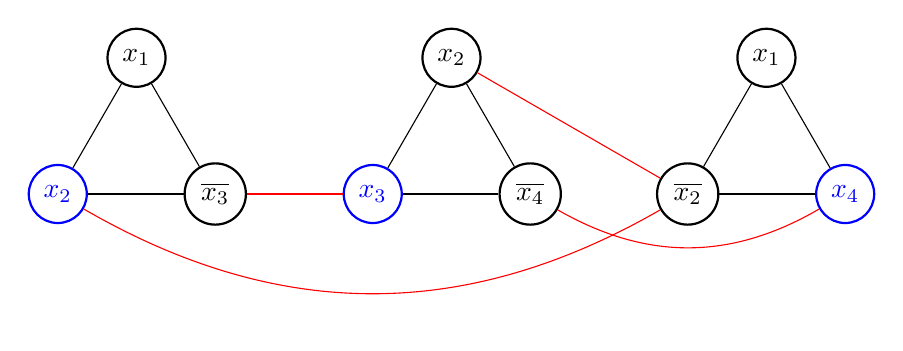
\begin{tikzpicture}
    \node[draw, circle, thick, blue] at (0, 0) (v1) {$x_2$};
    \node[draw, circle, thick] at (2, 0) (v2) {$\overline{x_3}$};
    \node[draw, circle, thick, blue] at (4, 0) (v3) {$x_3$};
    \node[draw, circle, thick] at (6, 0) (v4) {$\overline{x_4}$};
    \node[draw, circle, thick] at (8, 0) (v5) {$\overline{x_2}$};
    \node[draw, circle, thick, blue] at (10, 0) (v6) {$x_4$};
    \node[draw, circle, thick] at (1, 1.73) (v7) {$x_1$};
    \node[draw, circle, thick] at (5, 1.73) (v8) {$x_2$};
    \node[draw, circle, thick] at (9, 1.73) (v9) {$x_1$};

    \draw (v1) -- (v2);
    \draw (v1) -- (v7);
    \draw (v2) -- (v7);
    \draw[red] (v2) -- (v3);
    \draw (v3) -- (v4);
    \draw (v3) -- (v8);
    \draw (v4) -- (v8);
    \draw[red] (v5) -- (v8);
    \draw (v5) -- (v6);
    \draw (v5) -- (v9);
    \draw (v6) -- (v9);
    \draw[red] (v1) to[bend right] (v5);
    \draw[red] (v4) to[bend right] (v6);
\end{tikzpicture}
\end{center}
\begin{itemize}
    \item Red edges are edges connecting the same variables. 
    \item Blue nodes are those we can select as part of our independent set.
    \item The set of nodes we select as our independent set are the variables we set to true in 3SAT in order to satisfy it.  
    \item The 3SAT problem is satisfied if and only if our independent set is equal to the number of clauses.  (In this case, 3 clauses means we select three nodes.)  Our selected nodes represent the variable in each clause that is true.
\end{itemize}

\subsubsection*{Proving Hamiltonian Cycle is NP-Hard}
Given a directed graph $G$, is there a \underline{cycle} that visits each vertex exactly once?  The theorem says Hamiltonian Cycle is NP-complete, but we can prove that.  To do this, we build the following construction.
\begin{center} 
	\includegraphics*[width=0.8\textwidth]{W14_1.png} 
\end{center}
Each variable in 3-SAT gets a row of nodes, doubly linked.  The length of the row of nodes is $2 \times n + 2$, where $n$ is the number of clauses in 3-SAT.  Each start point and end point of each row is connected to both the start point and end point of the next row.  At this point, the Hamiltonian cycle must traverse across each row, in either the forwards or backwards direction.\\\\
Now, we link each clause into the graph.  For each clause, $c_i$, if it uses a given variable $x_j$, then add an edge going from $x_{j, 2i}$ to $c_i$, and an edge from $c_i$ to $x_{j, 2i + 1}$.  If the clause uses the complement of a variable, ($x_j$ is negated), then draw the edges in the reverse direction, from $x_{j, 2i + 1}$ to $c_i$ and from $c_i$ to $x_{j, i}$.  Each clause gets two columns on the graph to link to its variables.\\\\
A Hamiltonian Cycle passing through this graph would be required to pass through each clause at least once.  If a Hamiltonian Cycle exists in this graph, it gives the variable assignments necessary to satisfy every clause.  Moving from left to right in a variable's row corresponds to it being assigned to True, and moving backwards corresponds to it being assigned to False.

\subsection*{Proving Hamiltonian Path is NP-Hard}
We can prove Hamiltonian Path from Hamiltonian Cycle very easily.  Given a graph $G$ for Hamiltonian Cycle, if there exists a cycle, then every node must have one incoming edge and one outgoing edge.  Based on this fact, we simply pick any node, $i$, and separate it into two nodes.  One node, $i_i$ will contain all the incoming edges of $i$, and the other, $i_o$ will contain all the outgoing edges of $i$.  When given to the Hamiltonian Path solver, it will be forced to start a path at $i_o$ and end at $i_i$.  If the path does not exist, then the cycle must not exist either.  To retrieve the solution for the Cycle, connect the start and end points of the graph.

\subsection*{Traveling Salesman Problem}
Given $n$ cities, distances $d(i, j)$ between them, does there exist a path of length less than $k$ that visits every city exactly once, and returns home?  Importantly, the distance function need not satisfy the triangle inequality, and $d(i, j)$ need not equal $d(j, i)$.\\\\
To prove that, we can do a reduction from Hamiltonian Cycle.  However, we need a lemma first.  Let $G = (V, E)$ and $D = (V, d(i, j))$, where all distances are either $1$ or $2$.  $1$ if an edge exists between the two cities, $2$ otherwise.\\\\
\textbf{Lemma:} $G$ has a Hamiltonian Cycle if and only if $D$ has a tour of length $\leq$ n.\\\\
\textit{Proof.}  
If $G$ has a Hamiltonian Cycle, that is an ordering of the cities giving a tour in $D$ of length $n$.  Therefore, the forward implication is proven.\\
Suppose $D$ has a tour of length $\leq n$.  Then, the tour cannot use a distance-2 connection because with $n$ steps, that would be too long.  Therefore, it visits cities only on distance-1 edges which in $G$ are nodes with edges.\\\\
Thus, Hamiltonian cycle reduces to TSP, and TSP is NP-hard.



\end{document}